\begin{tabular}{M{7.5cm}M{10.5cm}}
	\textbf{LỚP CÔ THẢO - THẦY SANG}& \textbf{ĐỀ ÔN TẬP KIỂM TRA CUỐI HỌC KÌ 1}\\
	\textbf{MÃ ĐỀ: 001}& \textbf{Bài thi môn: VẬT LÝ 12}\\
	\textit{(Đề trường THCS-THPT Nguyễn Khuyến năm học 2024 -2025)}& \textit{Thời gian làm bài: 50 phút, không kể thời gian phát đề}
	
	\noindent\rule{4cm}{0.8pt} \\
\end{tabular}
\setcounter{section}{0}
\section{Câu trắc nghiệm nhiều phương án lựa chọn}
\textit{Thí sinh trả lời từ câu 1 đến câu 18. Mỗi câu hỏi thí sinh chọn một phương án}
\setcounter{ex}{0}
\Opensolutionfile{ans}[ans/FINAL-SEM1-001-TN]
% ===================================================================
\begin{ex}
	Nội năng của một vật
	\choice
	{là tổng động năng của các phân tử tạo nên vật}
	{chỉ phụ thuộc vào nhiệt độ của vật}
	{chỉ phụ thuộc vào thể tích của vật}
	{\True phụ thuộc vào thể tích và nhiệt độ của vật}
	\loigiai{}
\end{ex}
% ===================================================================
\begin{ex}
	Chọn câu đúng. Trong quá trình nóng chảy của nước đá đến khi nóng chảy hoàn toàn thì nhiệt độ của nước đá 
	\choice
	{luôn giảm.}
	{\True không thay đổi}
	{luôn tăng}
	{tăng lên sau đó giảm xuống}
	\loigiai{}
\end{ex}
% ===================================================================
\begin{ex}
	Cồn y tế chuyển từ thể lỏng sang thể khí rất nhanh ở điều kiện thông thường. Khi xoa cồn vào da, ta cảm thấy lạnh ở vùng da đó vì
	\choice
	{\True cồn thu nhiệt lượng từ cơ thể qua chỗ da đó để bay hơi}
	{cồn khi bay hơi tỏa nhiệt lượng vào chỗ da đó}
	{cồn khi bay hơi kéo theo lượng nước chỗ da đó ra cơ thể}
	{cồn khi bay hơi tạo ra dòng nước mát chỗ da đó}
	\loigiai{}
\end{ex}
% ===================================================================
\begin{ex}
	Nhiệt hóa hơi riêng có đơn vị đo là
	\choice
	{$\si{J/kg\cdot K}$}
	{$\si{g/mol}$}
	{$\si{mol}$}
	{\True $\si{J/kg}$}
	\loigiai{}
\end{ex}
% ===================================================================
\begin{ex}
	Ở những ngày rất lạnh, nhiều khu vực ở nước ta như Sapa, Mẫu sơn, nước có thể bị đóng băng. Hiện tượng này thể hiện sự chuyển thể nào của chất?
	\choice
	{Sự ngưng tụ}
	{\True Sự đông đặc}
	{Sự nóng chảy}
	{Sự hóa hơi}
	\loigiai{}
\end{ex}
% ===================================================================
\begin{ex}
	Nhiệt hóa hơi riêng là thông tin cần thiết trong việc thiết kế thiết bị nào dưới đây
	\choice
	{\True Tủ lạnh}
	{Máy sấy tóc}
	{Bàn là}
	{Nhiệt kế}
	\loigiai{}
\end{ex}
% ===================================================================
\begin{ex}
	Một lượng khí lí tưởng xác định ở trạng thái có áp suất $p_1$, thể tích $V_1$ và nhiệt độ tuyệt đối $T_1$. Thực hiện quá trình biến đổi lượng khí trên đến trạng thái có áp suất $p_2$, thể tích $V_2$ và nhiệt độ tuyệt đối $T_2$. Phương trình nào sau đây là đúng?
	\choice
	{\True $\dfrac{p_1V_1}{T_1}=\dfrac{p_2V_2}{T_2}$}
	{$\dfrac{p_1}{p_1}=\dfrac{V_1}{V_2}$}
	{$\dfrac{V_1}{V_2}=\dfrac{T_1}{T_2}$}
	{$\dfrac{p_1}{p_2}=\dfrac{T_1}{T_2}$}
	\loigiai{}
\end{ex}
% ===================================================================
\begin{ex}
	Chất nào sau đây có thể tồn tại ở cả ba thể rắn, lỏng, khí ở điều kiện tự nhiên trên trái đất
	\choice
	{Carbon dioxide}
	{Nitrogen}
	{\True Nước}
	{Oxygen}
	\loigiai{}
\end{ex}
% ===================================================================
\begin{ex}
	\immini{Cho một quá trình biến đổi trạng thái của một lượng khí xác định được biểu diễn như hình vẽ. Các thông số trạng thái áp suất p, thể tích V và nhiệt độ tuyệt đối T thay đổi như thế nào khi chuyển từ trạng thái (1) sang trạng thái (2)  
		\choice
		{T không đổi, V tăng và p tăng}
		{\True p tăng, V tăng và T tăng}
		{p tăng, V tăng và T giảm}
		{V không đổi, p tăng và T tăng}} 
	{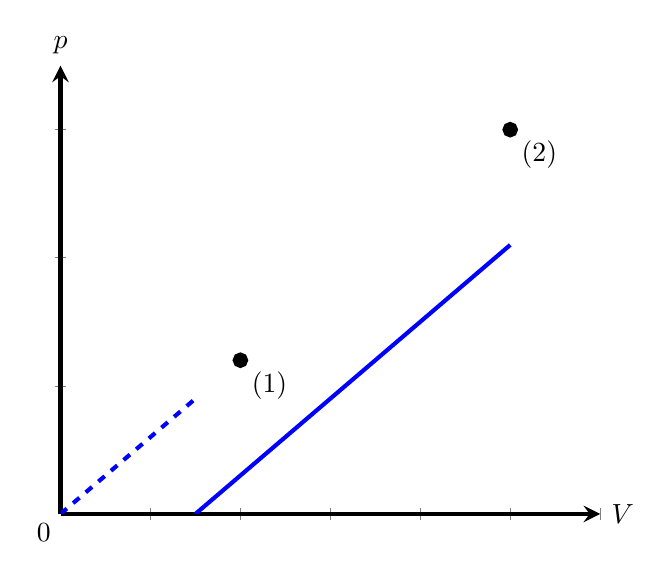
\begin{tikzpicture}  
			\begin{axis}[  ultra thick,
				xmin=0,  
				xmax=12,  
				ymin=0,  
				ymax=7, 
				samples=300,
				yticklabels=\empty,
				xticklabels=\empty,
				axis lines=center, 
				xlabel=$V$, 		ylabel=$p$,
				every axis y label/.style={at=(current axis.above origin),anchor=south},  
				every axis x label/.style={at=(current axis.right of origin),anchor=west},  ]
				\addplot [line width=1.5pt, blue, smooth, dashed, domain=0:3] {0.6*x};  
				\addplot [line width=1.5pt, blue, smooth, domain=3:10] {0.6*(x-3)};
				\filldraw (axis cs: 4,2.4) circle (2pt) node[below right] {(1)};
				\filldraw (axis cs: 10,6) circle (2pt) node[below right] {(2)};
				\coordinate (O) at (axis cs: 0,0);
			\end{axis}  
			\node[below left] at (O) {0};
	\end{tikzpicture}}
	\loigiai{}
\end{ex}
% ===================================================================
\begin{ex}
	Nhiệt nóng chảy riêng của một chất được kí hiệu $\lambda$ và có đơn vị $\dfrac{J}{kg}$. Nhiệt lượng cần thiết để làm nóng chảy hoàn thoàn $\xsi{m}{\left(\kilogram\right)}$ chất đó ở nhiệt độ nóng chảy là 
	\choice
	{$Q=\dfrac{\lambda}{m}$}
	{$Q=(m+\lambda)$}
	{$Q=\dfrac{m}{\lambda}$}
	{\True $Q=m\lambda$}
	\loigiai{}
\end{ex}
% ===================================================================
\begin{ex}
	Chọn phát biểu sai khi nói quá trình đẳng tích (thể tích của khối khí được giữ không đổi) của một lượng khí nhất định.
	\choice
	{\True Tích áp suất và nhiệt độ tuyệt đối là một hằng số}
	{Đồ thị mối liên hệ giữa áp suất và nhiệt độ tuyệt đối có dạng là đường thẳng}
	{Áp suất tỉ lệ thuận với nhiệt độ tuyệt đối}
	{Thương số giữa áp suất và nhiệt độ tuyệt đối là một hằng số}
	\loigiai{}
\end{ex}
% ===================================================================
\begin{ex}
	Câu nào sau đây là sai khi nói về quá trình đẳng nhiệt của một lượng khí nhất định?
	\choice
	{\True Khi áp suất khí tăng 2 lần thì thể tích cũng tăng 2 lần}
	{Đường biểu diễn áp suất theo thể tích là một phần của hyperbol}
	{Tích của áp suất và thể tích luôn không đổi}
	{Áp suất và thể tích tỉ lệ nghịch với nhau}
	\loigiai{}
\end{ex}
% ===================================================================
\begin{ex}
	Ở độ cao 11,5 $\si{km}$ nhiệt độ không khí là $\SI{-56}{\celsius}$ và khối lượng riêng của không khí $\mu = \SI{28.8E-3}{\kg/mol}$. Xem không khó ở độ cao này như khí lí tưởng có hằng số $R=\SI{8.31}{J/mol\cdot K}$. Âp suất khí quyển ở độ cao này là
	\choice
	{$\SI{21.36}{\kPa}$}
	{$\SI{22.80}{\kPa}$}
	{$\SI{21.64}{\kPa}$}
	{\True $\SI{22.54}{\kPa}$}
	\loigiai{$\dfrac{p}{DT}=\dfrac{R}{M}$ \Rightarrow $p\approx \SI{22.54E3}{Pa}$ }
\end{ex}
% ===================================================================
\begin{ex}
	Một khối khí lí tưởng chứa trong một xilanh có pit-tông chuyển động được. Lúc đầu khối khí có thể tích $\SI{18}{\dm^3}$, áp suất $\SI{1.5E5}{\Pa}$. Khối khí được làm lạnh đẳng áp cho đến khi thể tích còn $\SI{18}{\dm^3}$. Bỏ qua ma sát giữa pit-tông và xilanh. Công mà khối khí nhận được là
	\choice
	{$\SI{760}{\J}$}
	{$\SI{580}{\J}$}
	{\True $\SI{600}{\J}$}
	{$\SI{820}{\J}$}
	\loigiai{$A = p(V_1 - V_2) = \SI{600}{\J}$}
\end{ex}
% ===================================================================
\begin{ex}
	\immini{Hình bên là đồ thị biểu diễn sự phụ thuộc của áp suất (p) theo thể tích (V) của một lượng khí lí tưởng xác định khi giữ nhiệt độ không thay đổi. Khi thể tích khối khí là $\SI{0.64}{m^3}$ thì áp suất nhận giá trị nào dưới đây?
		\choice
		{$\SI{18.75}{\kPa}$}
		{\True $\SI{12.5}{\kPa}$}
		{$\SI{15.5}{\kPa}$}
		{$\SI{6.25}{\kPa}$}}
	{\includegraphics[scale=0.6]{../figs/FINAL_SEM1_001_2}}
	\loigiai{$p\cdot 0,64 = 20\cdot 0,4 \Rightarrow p = \SI{12.5}{kPa}$}      
\end{ex}
% ===================================================================
\begin{ex}
	Để mở nút chai bị kẹt, một người dùng cách hơ nóng khí trong chai. Biết rằng khí trong chai lúc chưa hơ nóng có áp suất bằng với áp suất khí quyển và bằng $\SI{1.0E5}{\Pa}$ và nhiệt độ $\SI{8.0}{\celsius}$. Để làm đẩy được nút chai ra cần có chênh lệch áp suất giữa khí trong chai và bên ngoài là $\SI{0.8E5}{\Pa}$. Người này cần hơ để khí trong chai nóng đến nhiệt độ thấp nhất là bao nhiêu ($\si{\celsius}$) để nút chai bật ra. Kết quả làm tròn đến hàng đơn vị.
	\choice
	{265}
	{248}
	{\True 233}
	{235}
	\loigiai{$\dfrac{10^5}{281,15}=\dfrac{1,8 \cdot 10^5}{T_2} \Rightarrow T_2 \approx \SI{506}{\K}$}
\end{ex}
% ===================================================================
\begin{ex}
	Nhiệt nóng chảy riêng của nước đá là $\SI{334E3}{\J/Kg}$. Năng lượng được hấp thụ bởi $\SI{10.0}{\g}$ nước đá để chuyển hoàn toàn từ thể rắn sang thể lỏng là
	\choice
	{$\SI{3.34E2}{\J}$}
	{$\SI{334E3}{\J}$}
	{$\SI{334E2}{\J}$}
	{\True $\SI{3340}{\J}$}
	\loigiai{}
\end{ex}
% ===================================================================
\begin{ex}
	Ở $\SI{27}{\celsius}$ thể tích của một lượng khí lí tưởng là 10,0 lít. Thể tích của lượng khí đó tăng thêm bao nhiêu lít nếu nung nóng đẳng áp để nhiệt độ khối khí tăng thêm $\SI{120}{\celsius}$? 
	\choice
	{3,1 lít}
	{\True 4,0 lít}
	{14,01 lít}
	{1,46 lít}
	\loigiai{}
\end{ex}
\Closesolutionfile{ans}
\section{Câu trắc nghiệm đúng/sai} 
\textit{Thí sinh trả lời từ câu 1 đến câu 4. Trong mỗi ý \textbf{a)}, \textbf{b)}, \textbf{c)}, \textbf{d)} ở mỗi câu, thí sinh chọn đúng hoặc sai}
\setcounter{ex}{0}
\Opensolutionfile{ans}[ans/FINAL-SEM1-001-TF]
% ===================================================================
\begin{ex}
	\immini{Làm thí nghiệm khảo sát mối liên hệ giữa thể tích và nhiệt độ của một lượng khí xác định khi giữ áp suất không đổi. Biết áp kết (1) có mức 0 ứng với áp suất khí quyển, đơn vị đo của áp kế là Bar ($\SI{1}{Bar}=\SI{E5}{Pa}$) ; xilanh (2); pit-tông (3) gắn với tay quay (4); hoopk chứa nước nóng (5) và cảm biến nhiệt (6). Đổ nước nóng vào hộp chứa cho ngập toàn xilanh. Dịch chuyển xilanh từ từ sao cho số chỉ của áp kế không đổi. Kết quả đo giá trị của phần thể tích chứa khí và nhiệt độ sau mỗi phút như bảng bên.}
	{\includegraphics[scale=1]{../figs/FINAL_SEM1_001_3}}
	\choiceTF[t]
	{\True Tỉ số $\dfrac{V}{t+273}$ trong 4 lần đo xấp xỉ bằng nhau, khi đó ta có kết luận $\dfrac{V}{t+273}=$ hằng số}  
	{Đồ thị biểu diễn sự phụ thuộc của thể tích V vào nhiệt độ t (\si{\celsius}) trong hệ trục (OtV) là đường thẳng đi qua gốc tọa độ O}
	{\True Mật độ phân tử trong khí xilanh giảm khi nhiệt độ của khối khí tăng}
	{\True Khi tăng nhiệt độ từ $\SI{32}{\celsius}$ $\SI{32}{\celsius}$ thì thể tích khí tăng thêm xấp xỉ $\SI{20}{\ml}$} 
	\loigiai{
		\begin{itemchoice}
			\itemch Đúng
			\itemch Sai. Nhiệt độ t ($\si{\celsius}$) thì không đi qua gốc tọa độ.
			\itemch Đúng. Khi T tăng thì V tăng mà số phân tử N không đổi nên mật độ phân tử giảm.
			\itemch Đúng. $\dfrac{72}{32+273}=\dfrac{V}{117+273} \Rightarrow V \approx \SI{72}{\ml} \Rightarrow \Delta V = \SI{20}{\ml}$
		\end{itemchoice}
	}
\end{ex}
\begin{ex}
	\immini{Một lượng khí lí tưởng ở trạng thái (1) có áp suất $\SI{4.5E5}{Pa}$, thể tích 1,5 lít và nhiệt độ $\SI{25}{\celsius}$. Khối khí này thực hiện một chu trình biến đổi từ trạng thái (1) đến trạng thái (2) (đường biểu diễn là một phần hyberlbol) rồi đén trạng thái (3), sau đó trở về trạng thái (1) như hình vẽ.}
	{\vspace{-0.5cm}\includegraphics[scale=0.8]{../figs/FINAL_SEM1_001_4}}
	\choiceTF[t]
	{\True Nhiệt độ khối khí ở trạng thái (2) là $\SI{25}{\celsius}$}
	{Từ trạng thái (3) trở về trạng thái (1) là quá trình đẳng áp}
	{\True Thể tích khối khí ở trạng thái (2) là 4,5 lít}
	{Từ trạng thái (2) chuyển đến trạng thái (3) nội năng của khí giảm một lượng $\SI{450}{\J}$}
	\loigiai{
		\begin{itemchoice}
			\itemch Đúng
			\itemch Sai. (3) sang (1) là đẳng tích.
			\itemch Đúng. $4,5 \cdot 10^5 \cdot 1,5 = 1,5 \cdot 10^5 V_2 \Rightarrow V_2 = 4,5l $.
			\itemch Sai. $U_{23}=\dfrac{i}{2}nR(T_2-T_1)=\dfrac{i}{2}\cdot1,5\cdot 10^5 \cdot (1,5-4,5)\cdot 10^{-3}=\dfrac{i}{2}\cdot \SI{450}{\J}$.
			\\ với $i \geq 3 \Rightarrow \Delta U \leq \SI{-675}{\J}$.
		\end{itemchoice}
	}
\end{ex}
\begin{ex}
	Một lốp ô tô được bơm căng không khí ở nhiệt độ $\SI{27}{\celsius}$. Áp suất ban đầu của khí ở áp suất khí quyển thường là $\SI{1.013E5}{Pa}$. Trong quá trình bơm, không khó vào trong lốp bị nén lại và giảm $\SI{75}{\percent}$ thể tích ban đầu (thể tích lượng khí trước khi bơm vào lốp), nhiệt độ khí trong lốp tăng đến $\SI{42}{\celsius}$.
	\choiceTF[t]
	{Trong suốt quá trình bơm, áp suất khí trong lốp xe không đổi}
	{\True Tỉ số thể tích của khí trước khi bơm vào lốp và thể tích sau khi bơm vào lốp là 4}
	{Cần bơm lốp xe với lượng khí lớn nhất để phần diện tích tiếp xúc giữa lốp xe với mặt đường nhỏ nhất, khi đó ma sát giữa lốp xe và mặt đường là nhỏ nhất}
	{\True Khi ô tô chạy với tốc độ cao, nhiệt độ không khí trong lốp tăng đến $\SI{74.6}{\celsius}$ và thể tích lốp thăng thêm $\SI{2}{\percent}$ so với thể tích lốp khi nhiệt độ $\SI{42}{\celsius}$. Áp suất khí trong lốp lúc này là xấp xỉ bằng $\SI{460.3}{kPa}$}
	\loigiai{
		{\includegraphics[scale=2]{../figs/FINAL_SEM1_001_7}}
		\\ $\dfrac{1,013 \cdot 10^5 \cdot V_1}{300,15}=\dfrac{p_2 \cdot 0,25V_1}{315,15}= \dfrac{p_3 \cdot 0,255V_1}{347,75}
		\\ \Rightarrow \begin{cases}
			p_2 \approx \SI{425E3}{\Pa}\\ p_1 \approx \SI{460.3E3}{\Pa}
		\end{cases}$
	}
\end{ex}
\begin{ex}
	Bóng thám không là một thiết bị được sử dụng phổ biến trong ngành khí tượng để thu thập dữ liệu về các thông số thời tiết như nhiệt độ, độ ẩm, áp suất và hướng gió ở độ cao khác nhau của bầu khí quyển. Trên quả bóng có gắn thiết bị gọi là Radiosonde có chức năng ghi nhận các dữ liệu thông qua các cảm biến và phát tín hiệu radio để truyền dữ liệu trở lại mặt đất để các nhà khoa học và nhà khí tượng có thể thu nhập thông tin và phân tích. Bóng thám không thường được làm từ các vật liệu nhẹ có khả năng chịu biến dạng.
	\choiceTF[t]
	{\True Bóng được bơm khí nhẹ như hydrogen hoặc helium}
	{Càng lên cao nhiệt độ của không khí trong bóng càng tăng làm áp suất bóng tăng và bóng sẽ nổ}
	{Bóng thường làm từ các vật liệu nhẹ và có độ bền cao như hợp kim của nhôm hoặc composite}
	{\True Một quả bóng thám không dự báo thời tiết sẽ bị nổ ở áp suất $\SI{0.04}{atm}$ và thể tích tăng lên đến $\SI{542.5}{cm^3}$. Khi ở mặt đất có nhiệt độ $\SI{27}{\celsius}$, bơm khí nhẹ vào bóng với áp suất $\SI{1}{atm}$, thể tích của bóng là $\SI{30}{cm^3}$. Nhiệt độ ở độ cao mà khi bóng nổ là $\SI{-56}{\celsius}$}
	\loigiai{
		\begin{itemchoice}
			\itemch Đúng
			\itemch Sai. Càng lên cao nhiệt độ càng giảm và áp suất bên ngoài cũng giảm. Nhưng áp suất bên ngoài giảm nhanh hơn áp suất bên trong làm bóng nở ra vượt quá giới hạn chịu đựng của vật liệu dẫn đến bóng sẽ nổ.
			\itemch Sai. Bóng thám không thường được làm từ các vật liệu nhẹ có khả năng biến dạng tốt như sao su hoặc latex để bóng có thể giãn nở đến khi lên cao mà không bị nổ sớm.
			\itemch Đúng. $\dfrac{0,04 \cdot 542,5}{T}=\dfrac{1\cdot 30}{27+273} \Rightarrow T \approx \SI{217}{\K} \Rightarrow t \approx \SI{-56}{\celsius} $
		\end{itemchoice}
	}
\end{ex}

\Closesolutionfile{ans}
\section{Câu trắc nghiệm trả lời ngắn} \textit{Thí sinh trả lời từ câu 1 đến câu 6}
\setcounter{ex}{0}
\Opensolutionfile{ans}[ans/FINAL-SEM1-001-TL]
% ===============================================================
\begin{ex}
	Có bao nhiêu kilogam ($\si{\kg}$) khí oxygen (xem là khí lí tưởng) chứa trong bình cầu thể tích $\SI{200}{l}$ ở nhiệt độ $\SI{27}{\celsius}$ và áp suất khí trong bình $\SI{100}{kPa}$. Biết khí oxygen có khối lượng mol $\mu=\SI{32}{\g/mol}$, hằng số khí $R=\SI{8.31}{\J/mol\cdot K}$. Kết quả lấy đến hai chữ số thập phân sau dấu phẩy.
	\shortans[oly]{0,26}
	\loigiai{
		$\dfrac{pV}{T}=\dfrac{m}{M}R \Rightarrow \dfrac{100 \cdot 10^3 \cdot 200 \cdot 10^{-3}}{T} = \dfrac{m}{32 \cdot 10^{-3}}8,31 \Rightarrow m \approx \SI{0.26}{\kg}  $
	}
\end{ex}
\begin{ex}
	Biết nhiệt dung riêng của nước đá và nước lần lượt là $\SI{2100}{\J/Kg}$ và $\SI{4180}{\J/Kg}$, nhiệt nóng chảy riêng của nước đá là $\SI{3.33E5}{\J/kg}$ và nhiệt hóa hơi riêng của nước là $\SI{2.3E6}{\J/kg}$. Nhiệt lượng cần thiết để làm $\SI{2.0}{\g}$ nước đá ở $\SI{-20}{\celsius}$ chuyển hoàn toàn thành hơi nước ở $\SI{100}{\celsius}$ là bao nhiêu kilojun ($\si{kJ}$). Kết quả lấy đến một chữ số thập phân sau dấu phẩy.
	\shortans[oly]{6,2 }
	\loigiai{
		$Q=m(c_d \cdot \Delta t_d + \lambda + c_n \Delta t_n +L)=2 \cdot 10^{-3} \cdot (2100 \cdot 20 + 3,33 \cdot 10^5 + 4180 \cdot 100 + 2,3 \cdot 10^6) = \SI{6186}{\J}$
	}
\end{ex}
\begin{ex}
	\immini{Dùng 1 bơm hút có thể tích xilanh là $\SI{150}{cm^3}$ để hút không khí từ một bình có thể tích $V=\SI{2}{l}$ (kể cả ống nối giữa bơm và bình) chứa không khí ở áp suất $p_0=\SI{E5}{Pa}$. Coi quá trình trên nhiệt độ của khí không thay đổi. Áp suất khí trong bình sau 8 lần hút là bao nhiêu $\si{kPa}$? Kết quả lấy đến một chữ số thập phân sau dấu phẩy.} 
	{\includegraphics[scale=0.7]{../figs/FINAL_SEM1_001_5}}
	\shortans[oly]{56,1 }
	\loigiai{
		$\begin{cases}
			p_0V=p_1\left(V+V_0\right)\\
			p_1V=p_2\left(V+V_0\right)\\
			\dots\\
			p_7V=p_8\left(V+V_0\right)
		\end{cases}$\\
		Nhân các vế rồi rút gọn được $p_0V^8=p_8(V+V_0)^8$
		\\ $10^5 \cdot 2^8 = p_8 \cdot (2+0,15)^8 \Rightarrow p_8 \approx \SI{56070}{\Pa} $
	}
\end{ex}
\begin{ex}
	Một bóng đèn dây tóc có thể tích chứa đầy khí trơ (xem như khí lí tưởng). Khi đèn không hoạt động có nhiệt độ $\SI{27}{\celsius}$, áp suất khí trong bóng đèn là $\SI{1.65}{atm}$ . Khi đèn hoạt động bình thường, nhiệt độ của bóng đèn đạt $\SI{329}{\celsius}$. Áp suất của khối khí trong bóng đèn khi đèn hoạt động bình thường là bao nhiêu? Cho rằng thể tích của bóng đèn không thay đổi theo nhiệt độ. Kết quả lấy đến hai chữ số thập phân sau dấu phẩy.
	\shortans[oly]{3,31}
	\loigiai{
		$\dfrac{1,65}{27+273}=\dfrac{p}{329+273} \Rightarrow p \approx \SI{3.31}{atm}$
	}
\end{ex}
\begin{ex}
	PSI là chỉ số áp suất của không khí bị nén trong lốp xe, được đo bằng đơn vị Pounds trên một Inch vuông (Pounds per Square Inch). PSI thường được ghi trên thành lốp xe, nó cho biết áp suất tối đa mà lốp xe chịu được. Khi bơm hoặc kiểm tra lốp, chúng ta phải làm sao cho lốp đủ hơi, tức là có đủ số PSI cần thiết, thiếu quá hoặc thừa quá đều có thể đưa đến tình trạng hại xe, hư lốp, hao mòn và nguy hiểm nhất là nổ lốp, gây ra tai nạn nghiêm trọng. Một chiếc lốp sau của xe VINFAST chứa không khí ở áp suất 40 Psi (đổi đơn vị $\SI{1}{Psi} \approx \SI{6895}{Pa}$ và nhiệt độ $\SI{27}{\celsius}$. Khi xe chạy nhanh, lốp xe nóng lên làm nhiệt độ không khí trong lốp xe tăng lên tới $\SI{57}{\celsius}$. Áp suất khí trong lốp ở nhiệt độ này là bao nhiêu Psi
	\shortans[oly]{44 }
	\loigiai{
		$\dfrac{40}{27+273}=\dfrac{p}{57+273} \Rightarrow p = \SI{44}{Psi}.$
	}
\end{ex}
\begin{ex}
	\immini{Có một lượng khí helium chứa trong xi lanh đậy kín bởi pít tông (xem như khí lí tưởng) biến đổi chậm từ trạng thái (1) đến trạng thái (2). Hình bên là đường biểu diễn sự phụ thuộc áp suất theo thể tích của khối khí. Khối khí đã nhận một công bằng bao nhiêu kilojun (\si{\kJ}) kể từ lúc bắt đầu biến đổi trạng thái đến lúc đạt nhiệt độ cao nhất.Biết $\SI{1}{atm}$ = \SI{1.013E5}{Pa}. Kết quả lấy đến hai chữ số thập phân sau dấu phẩy.}
	{\vspace{-0.5cm}\includegraphics[scale=1.2]{../figs/FINAL_SEM1_001_6}}
	\shortans[oly]{7,60 }
	\loigiai{
		$p=aV+b\Rightarrow\begin{cases}
			15=10a+b\\
			5=30a+b
		\end{cases}\Rightarrow\begin{cases}
			a=\SI{-0.5}{atm/\liter}\\b=\SI{20}{atm}
		\end{cases}\Rightarrow p=-0,5V+20$\\
		$T_{\max}\Rightarrow pV=\left(-0,5V+20\right)V=-0,5V^2+20V$ đạt max tại $V=\dfrac{20}{2\cdot 0,5}=\SI{20}{\liter}\Rightarrow p=\SI{10}{atm}$\\
		Công khí nhận từ (1) đến khi nhiệt độ cao nhất là diện tích hình thang:
		$$A=\dfrac{1}{2}\left(p_1+p\right)\cdot\left(V_1-V\right)\approx\SI{7.60E3}{\joule}=\SI{7.60}{\kilo\joule}.$$
		
	}
\end{ex}

\Closesolutionfile{ans}
\begin{center}
	\textbf{--- HẾT ---}
\end{center}